%%%%%%%%%%%%%%%%%%%%%%%%%%%%%%%%%%%%%%%%%%%%%%%%%%%%%%%%%%%%%%%%%%%%%%%%%%%

\documentclass{standalone}

\usepackage{amsmath}
\usepackage{mathptmx}
\usepackage{pgfplots}
\usetikzlibrary{external}
\tikzexternalize{ecoli}
\pgfplotsset{compat=1.15}

%% IEEE uses Times Roman font, so we'll default to Times.
%% These three commands make up the entire times.sty package.
\renewcommand{\rmdefault}{ptm}
\renewcommand{\ttdefault}{pcr}
\normalfont\selectfont

\begin{document}

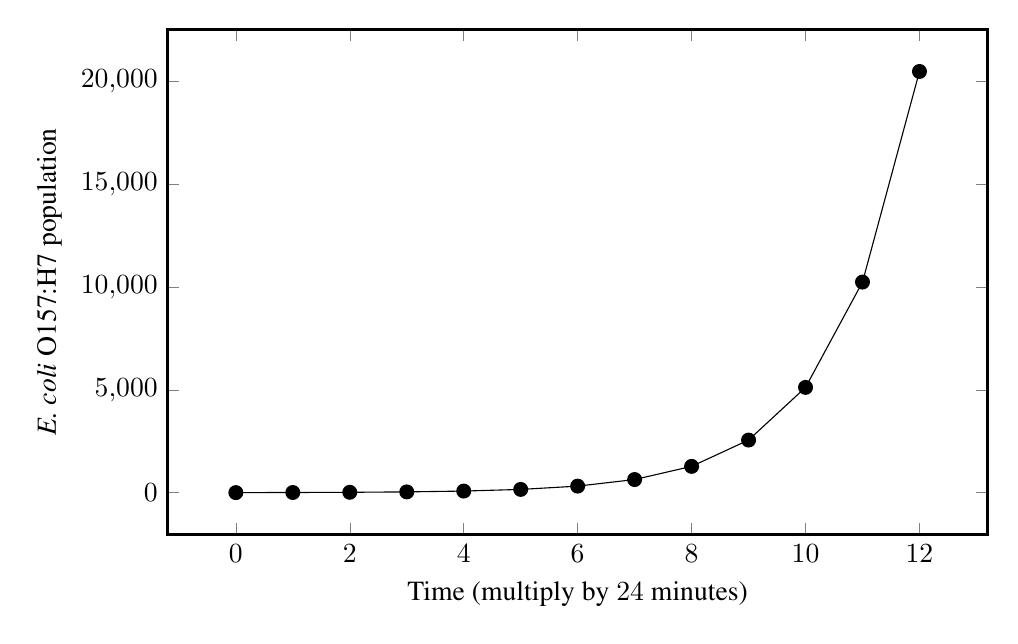
\begin{tikzpicture}
\tikzset{%%
  every mark/.append style={scale=1.0},%%
  scale=1.0%%
}
\pgfplotsset{%%
  every axis/.append style={font=\normalsize}%%
}
%%
\begin{axis}[%%
  axis line style=very thick,%%
  dotStyle/.style={mark size=2.5,black,mark color=black,mark=*},%%
  enlargelimits=true,%%
  height=8cm,%%
  width=12cm,%%
  %% x axis
  xlabel={\normalsize Time~(multiply by $24$ minutes)},%%
  %% y axis
  ylabel={\normalsize \emph{E.~coli} O157:H7 population},%%
  scaled y ticks=false,%%
  y tick label style=/pgf/number format/fixed%%
]
%%
%%
\addplot[dotStyle] coordinates {
  (0, 5)
  (1, 10)
  (2, 20)
  (3, 40)
  (4, 80)
  (5, 160)
  (6, 320)
  (7, 640)
  (8, 1280)
  (9, 2560)
  (10, 5120)
  (11, 10240)
  (12, 20480)
};
\end{axis}
\end{tikzpicture}

\end{document}
